\documentclass[9pt,twocolumn,twoside,]{pnas-new}

% Use the lineno option to display guide line numbers if required.
% Note that the use of elements such as single-column equations
% may affect the guide line number alignment.


\usepackage[T1]{fontenc}
\usepackage[utf8]{inputenc}

% tightlist command for lists without linebreak
\providecommand{\tightlist}{%
  \setlength{\itemsep}{0pt}\setlength{\parskip}{0pt}}


% Pandoc citation processing
%From Pandoc 3.1.8
% definitions for citeproc citations
\NewDocumentCommand\citeproctext{}{}
\NewDocumentCommand\citeproc{mm}{%
  \begingroup\def\citeproctext{#2}\cite{#1}\endgroup}
\makeatletter
 % allow citations to break across lines
 \let\@cite@ofmt\@firstofone
 % avoid brackets around text for \cite:
 \def\@biblabel#1{}
 \def\@cite#1#2{{#1\if@tempswa , #2\fi}}
\makeatother
\newlength{\cslhangindent}
\setlength{\cslhangindent}{1.5em}
\newlength{\csllabelwidth}
\setlength{\csllabelwidth}{3em}
\newenvironment{CSLReferences}[2] % #1 hanging-indent, #2 entry-spacing
 {\begin{list}{}{%
  \setlength{\itemindent}{0pt}
  \setlength{\leftmargin}{0pt}
  \setlength{\parsep}{0pt}
  % turn on hanging indent if param 1 is 1
  \ifodd #1
   \setlength{\leftmargin}{\cslhangindent}
   \setlength{\itemindent}{-1\cslhangindent}
  \fi
  % set entry spacing
  \setlength{\itemsep}{#2\baselineskip}}}
 {\end{list}}
\usepackage{calc}
\newcommand{\CSLBlock}[1]{#1\hfill\break}
\newcommand{\CSLLeftMargin}[1]{\parbox[t]{\csllabelwidth}{#1}}
\newcommand{\CSLRightInline}[1]{\parbox[t]{\linewidth - \csllabelwidth}{#1}\break}
\newcommand{\CSLIndent}[1]{\hspace{\cslhangindent}#1}


\templatetype{pnasresearcharticle}

\title{Rapport BIO500}

\author[]{Éloïse Paquette, Danaé Vaillancourt, Élodie Michel et Camille
Breton}



% Please give the surname of the lead author for the running footer
\leadauthor{}

% Please add here a significance statement to explain the relevance of your work
\significancestatement{}


\authorcontributions{}



\correspondingauthor{\textsuperscript{} }

% Keywords are not mandatory, but authors are strongly encouraged to provide them. If provided, please include two to five keywords, separated by the pipe symbol, e.g:


\begin{abstract}

\end{abstract}

\dates{This manuscript was compiled on \today}
\doi{\url{www.pnas.org/cgi/doi/10.1073/pnas.XXXXXXXXXX}}

\begin{document}

% Optional adjustment to line up main text (after abstract) of first page with line numbers, when using both lineno and twocolumn options.
% You should only change this length when you've finalised the article contents.
\verticaladjustment{-2pt}



\maketitle
\thispagestyle{firststyle}
\ifthenelse{\boolean{shortarticle}}{\ifthenelse{\boolean{singlecolumn}}{\abscontentformatted}{\abscontent}}{}

% If your first paragraph (i.e. with the \dropcap) contains a list environment (quote, quotation, theorem, definition, enumerate, itemize...), the line after the list may have some extra indentation. If this is the case, add \parshape=0 to the end of the list environment.

\acknow{}

\section*{Résumé}\label{ruxe9sumuxe9}
\addcontentsline{toc}{section}{Résumé}

À l'aide de R Studio et du langage SQL, des figures ont été créées à
partir d'une base de données sur les lépidoptères afin d'analyser
l'effet des variations temporelles et spatiales sur leurs communautés.
Après plusieurs analyses, on remarque une augmentation en richesse
spécifique au fil des générations, soit très forte après les années 2000
mais très variable en deçà, probablement par une fluctuation d'effort
d'échantillonnage ou par plusieurs pressions écologiques. Il y toutefois
une forte concentration de la richesse spécifique dans le sud de la
province du Québec et plus faible au nord, une hétérogénéité expliquée
par les gradients d'altitude et de climat. Enfin, la diversité des
espèces dans les dates d'arrivée et de départ suggère une niche
temporelle propre à chacune, aidant à la réduction de la compétition
interspécifique pour les ressources.

\section*{Introduction}\label{introduction}
\addcontentsline{toc}{section}{Introduction}

Au sein d'une communauté et d'un territoire, les espèces s'adaptent aux
nouvelles conditions et aux changements environnementaux sur une échelle
de temps variable. Les interactions entre les espèces peuvent alors
modifier la composition de la communauté et sa diversité (Nieto-Sánchez
et al., 2015). Cependant au sein de la famille des lépidoptères, comment
les variations spatiales et temporelles influencent-elles la structure
de leurs communautés ? Est-ce que certaines espèces seront impactées
plus que d'autres ?

\section*{Méthode}\label{muxe9thode}
\addcontentsline{toc}{section}{Méthode}

La base de données des lépidoptères est une liste d'observations de
différentes espèces de papillons, comprenant leur nom scientifique, la
date, le lieu où l'échantillon a été prélevé à l'aide de coordonnées
géographiques (latitude et longitude), l'heure, le jour et l'année
d'observation ainsi que tous les droits d'auteur, comprenant le
créateur, le titre, les licences, la source originale et le publicateur.
Cette dernière comprenant environ 441 891 observations et ce, sur un
intervalle de données allant de 1859 à 2023.

Afin de pouvoir utiliser cette base de données, nous avons procédé à une
revalidation en éliminant et triant les lacunes humaines potentielles
dans l'enregistrement des données à l'aide du logiciel R studio. Une
variété de tests a été exécuté pour parvenir à l'obtention de données
valides et d'une reproductibilité dans nos résultats. Des erreurs non
négligeables, comme des NA non-expliquer, des échantillons répétés, des
valeurs irréels dans les dates, les années, les heures et même les
coordonnées, devant être filtrer pour être des points seulement au
Québec, ont été corrigés et l'identification des bons types par colonnes
ont été modifiés.

Ensuite, une fois la base de données considérée comme valide, nous avons
pu procéder à la création de tables, avec l'aide du langage informatique
SQL, en regroupant les colonnes pertinentes ensembles, créer les liens
entre ces dernières et ainsi optimiser l'analyse de nos données. En
faisant des requêtes dans nos différentes tables, nous avons alors été
en mesure de créer des figures nous aidant à répondre à notre question
de départ. Finalement, une fois tous nos manipulations insérées dans des
scripts différents dans le logiciel R, nous avons procédé à
l'automatisation de notre code à l'aide du package Target et ainsi créer
une chaîne de traitement permettant à nos résultats d'être
reproductibles.

\section*{Résultats \& Discussion}\label{ruxe9sultats-discussion}
\addcontentsline{toc}{section}{Résultats \& Discussion}

\section*{Richesse spécifique à travers le
temps}\label{richesse-spuxe9cifique-uxe0-travers-le-temps}
\addcontentsline{toc}{section}{Richesse spécifique à travers le temps}

La richesse spécifique observée à travers le temps révèle une dynamique
marquée par une accélération récente. Pendant plus d'un siècle, la
richesse observée est demeurée faible et relativement constante, ce qui
pourrait s'expliquer par un effort d'échantillonnage limité ou des
lacunes dans l'enregistrement des données (Bowler et al., 2025). Ce
n'est qu'à partir des années 2000 que l'on observe une augmentation
brutale du nombre d'espèces recensées, comme le montrent la figure 1.
Cette tendance peut être liée à l'émergence de nouvelles technologies de
collecte de données (ex. plateformes participatives comme iNaturalist ou
eButterfly), à une mobilisation accrue des citoyens scientifiques, ainsi
qu'à une meilleure accessibilité des outils d'identification. Ces
facteurs peuvent conduire à une augmentation apparente de la richesse
spécifique, sans nécessairement refléter une transformation écologique
réelle des communautés (Bowler et al., 2025).

\begin{figure}[H]

{\centering 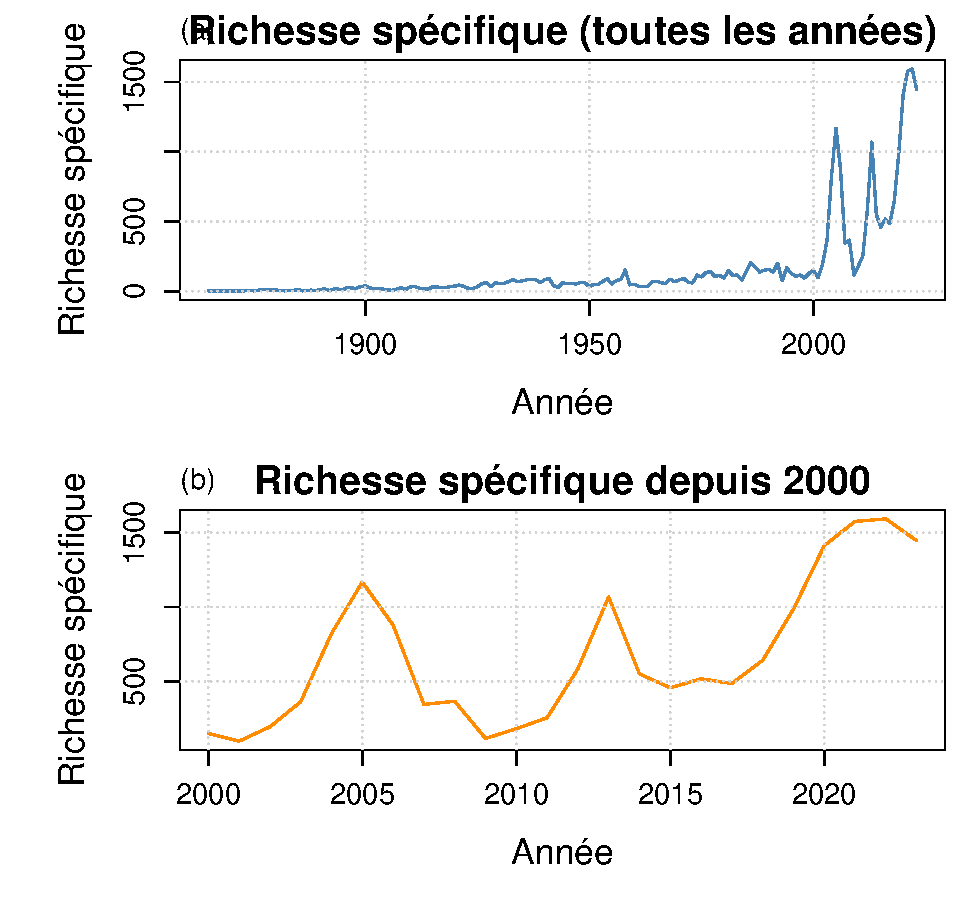
\includegraphics[width=0.8\linewidth]{rapport_final_BIO500_files/figure-latex/fig_richesse_temporelle-1} 

}

\caption{\label{fig:fig_richesse_temporelle}(a) Concentration en richesse spécifique des lépidoptères sur une échelle de temps comprise entre 1859 et 2023. (b) Concentration en richesse spécifique des lépidoptères sur une échelle de temps comprise entre 2000 et 2023.}\label{fig:fig_richesse_temporelle}
\end{figure}

Même si cette figure ne montre pas directement les variations spatiales,
la montée récente de la richesse spécifique pourrait aussi être le
reflet d'un élargissement spatial des efforts de surveillance.
L'intégration de nouveaux sites ou régions dans les bases de données
pourrait contribuer à accroître artificiellement la richesse observée à
l'échelle régionale.

La figure (b), centrée sur les données postérieures à l'an 2000, révèle
une forte variabilité interannuelle de la richesse spécifique, avec des
pics marqués autour de 2005, 2013 et 2021. Cette variabilité pourrait
être liée à des fluctuations dans l'effort d'échantillonnage, mais elle
pourrait aussi refléter des changements écologiques réels, notamment en
lien avec les effets du changement climatique sur la phénologie et la
distribution des espèces (Menéndez et al., 2006). L'augmentation
progressive observée vers 2020-2021 pourrait également coïncider avec
une hausse de la participation citoyenne à la collecte de données,
amplifiée par des plateformes comme iNaturalist. Ces résultats
soulignent l'importance de considérer les facteurs à la fois écologiques
et méthodologiques lorsqu'on interprète des tendances temporelles à
court terme.

Enfin, l'analyse temporelle longue permet de constater que la structure
des communautés n'est pas stable dans le temps, et qu'elle est soumise à
de multiples pressions, à la fois écologiques et méthodologiques. Ces
observations rappellent l'importance d'interpréter avec prudence les
tendances en biodiversité, surtout lorsque les données proviennent de
sources hétérogènes ou de périodes très contrastées en termes d'effort
d'observation (Bowler et al., 2025).

\section*{Richesse spécifique à travers
l'espace}\label{richesse-spuxe9cifique-uxe0-travers-lespace}
\addcontentsline{toc}{section}{Richesse spécifique à travers l'espace}

La carte de la richesse spécifique des lépidoptères au Québec (Figure 2)
illustre de façon marquée les variations spatiales dans la composition
des communautés. On remarque une très forte concentration de la richesse
spécifique dans le sud de la province. Ces zones coïncident largement
avec les régions les plus densément peuplées, les plus facilement
accessibles et les plus transformées par l'activité humaine (Québec,
2021). En revanche, la richesse spécifique diminue de manière marquée en
remontant vers le nord.

\begin{figure}[H]

{\centering 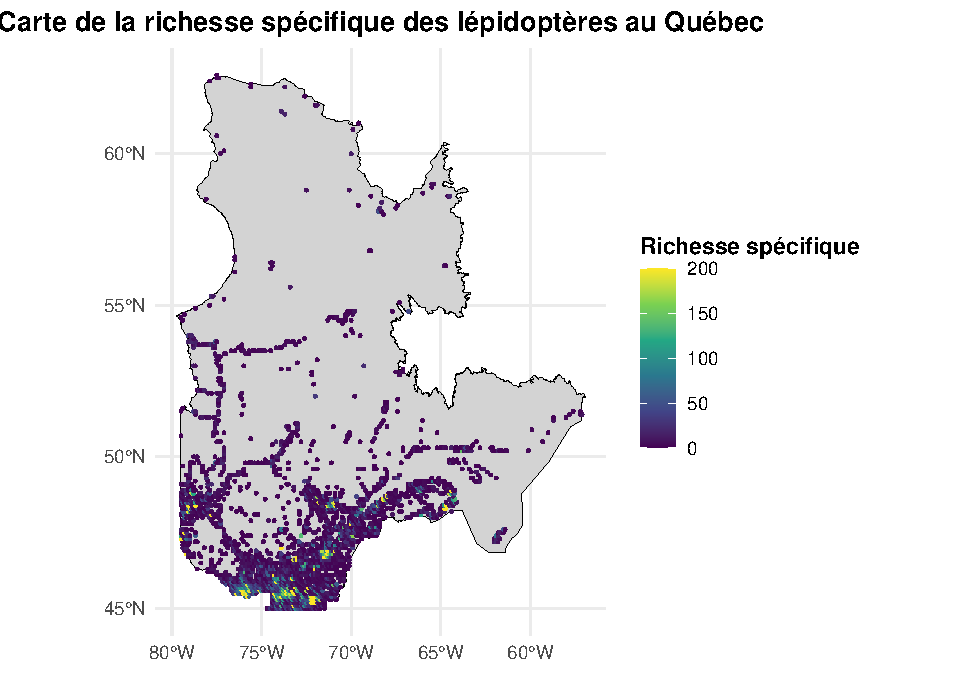
\includegraphics[width=0.7\linewidth]{rapport_final_BIO500_files/figure-latex/fig_richesse_spatiale-1} 

}

\caption{\label{fig:fig_richesse_spatiale}Carte du Québec représentant un gradient de concentrations en richesse spécifiques des lépidoptères, allant de 0 à 200, à la suite de l’échantillonnage sur une échelle de temps compris entre 1859 et 2023.}\label{fig:fig_richesse_spatiale}
\end{figure}

Plusieurs facteurs peuvent expliquer cette hétérogénéité. Sur le plan
écologique, les gradients de latitude, d'altitude et de climat
influencent la diversité des espèces : les milieux plus chauds et plus
diversifiés du sud offrent des conditions favorables à une plus grande
variété de lépidoptères (White et Kerr, 2006). De plus, les régions du
sud du Québec abritent une mosaïque d'habitats (zones agricoles, forêts
mixtes, milieux humides) propices à l'établissement d'un plus grand
nombre d'espèces.

Cette variation spatiale entraîne des structures de communautés très
contrastées entre les régions : dans le sud, la compétition entre
espèces peut être plus intense, avec des dynamiques de partage de niche
et de spécialisation plus complexes. À l'inverse, dans le nord, les
communautés sont probablement dominées par un nombre restreint d'espèces
généralistes, capables de tolérer des conditions plus rudes et de
coloniser des habitats plus homogènes.

Il faut cependant souligner que cette carte peut aussi refléter des
biais d'échantillonnage. Les zones plus accessibles ont historiquement
été davantage échantillonnées, ce qui peut amplifier artificiellement la
richesse apparente dans le sud. Il est donc important d'interpréter ces
résultats avec prudence et de compléter les analyses avec des données
d'effort d'échantillonnage si disponibles. En somme, la variation
spatiale influence profondément la structure des communautés de
lépidoptères au Québec, en déterminant à la fois la richesse spécifique,
la composition des espèces et les interactions écologiques entre elles.

\section*{Phénologie}\label{phuxe9nologie}
\addcontentsline{toc}{section}{Phénologie}

La figure 3 met en évidence la phénologie de la présence des espèces de
lépidoptères les plus observées au cours de l'année. Cette diversité
dans les dates d'arrivée et de départ suggère une niche temporelle
propre à chaque espèce, réduisant potentiellement la compétition
interspécifique pour les ressources (Ziv et Smallwood, 2000). Certaines
espèces, comme Plodia interpunctella, sont actives dès le mois de
janvier, alors que d'autres, telles que Acleris maccana, n'apparaissent
qu'en juin.

\begin{verbatim}
## Warning: Use of `summary_data$end_date` is discouraged.
## i Use `end_date` instead.
\end{verbatim}

\begin{figure}[H]

{\centering 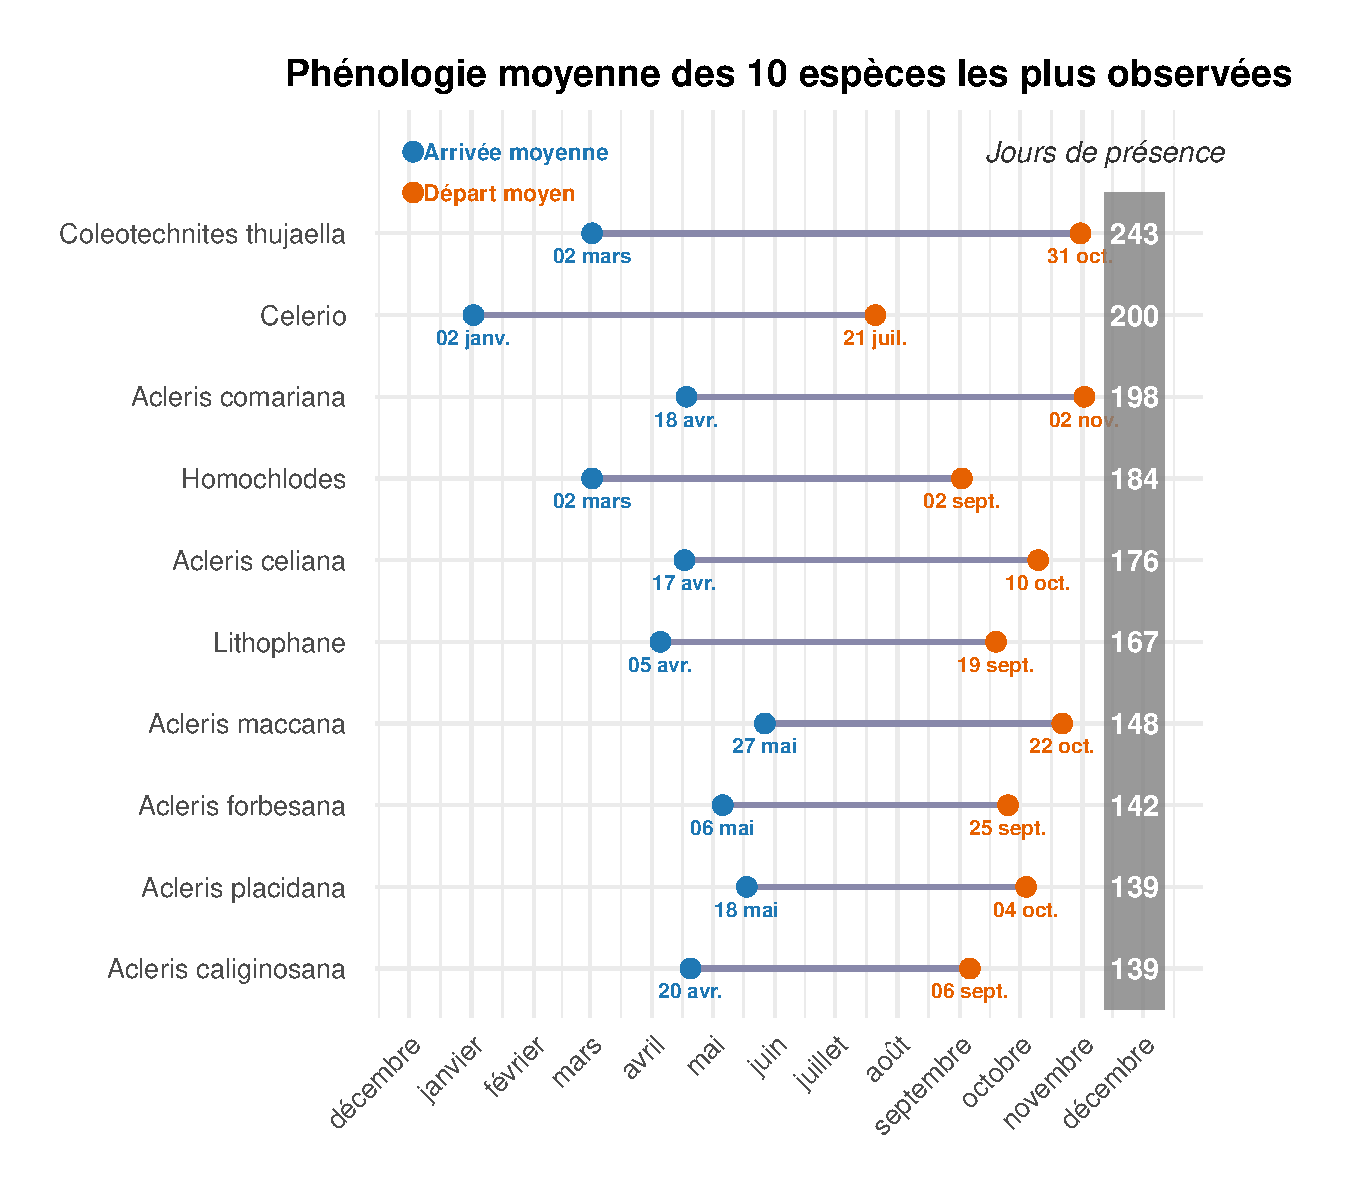
\includegraphics[width=0.8\linewidth]{rapport_final_BIO500_files/figure-latex/fig_phenologie-1} 

}

\caption{\label{fig:fig_phenologie}Variabilité temporelle de la présence des 10 espèces de lépidoptères les plus abondantes en comparant leurs dates d’arrivée et de départ durant une année complète.}\label{fig:fig_phenologie}
\end{figure}

On remarque également une forte variabilité dans la durée de présence,
allant de 127 jours pour certaines espèces à 243 jours pour
Coleotechnites thujaella. Cette disparité reflète probablement des
différences dans les stratégies de vie, les tolérances climatiques et
les cycles biologiques. En effet, la température est un facteur crucial
pour les ectothermes. Chez les insectes, comme les lépidoptères, qui,
par leur durée de développement généralement courte, vont avoir
plusieurs générations au cours de la saison, chacune soumise à des
conditions climatiques différentes (Gibert, 2012). Avec une hausse de la
température, les espèces moins plastiques, vont plutôt changer leur aire
de répartition en colonisant ou en abandonnant des habitats qui sont
devenus favorables ou défavorables. Tandis que les espèces à longue
durée de présence vont plutôt répondre à ces changements en modifiant la
phénologie de leur cycle de vie ou bien par une adaptation au milieu par
plasticité phénotypique. Ces différentes techniques dépendront de
l'importance du changement, l'échelle de temps considéré et les traits
d'histoire de vie des organismes (Gibert, 2012).

Les espèces présentent sur une longue durée pourraient alors jouer un
rôle structurant plus constant dans la communauté, alors que les espèces
plus éphémères pourraient avoir un impact plus ponctuel mais important
durant leur pic d'abondance. Les variations temporelles illustrées
influencent donc directement la structure des communautés, en affectant
les interactions écologiques (comme la compétition, la prédation ou la
pollinisation) et en modulant la diversité observée au fil des saisons.

\section*{Conclusion}\label{conclusion}
\addcontentsline{toc}{section}{Conclusion}

À la lumière des résultats obtenus, il est clair que les variations
spatiales et temporelles au fil des générations influencent la structure
des communautés de lépidoptères, en modifiant la dynamique de
concentration en richesse spécifique dans les différentes régions du
Québec ainsi que le temps de présence des espèces durant une année. Ces
variations s'expliquent majoritairement par les pressions écologiques et
environnementales, mais aussi par les fluctuations ou le manque d'effort
d'échantillonnage lors de la collecte de données par les chercheurs. Il
demeure que la réalité actuelle ne peut être ignorée : les hausses de
température, l'urbanisation croissante et la destruction des habitats
exigent une adaptation rapide des espèces (Gibert, 2012). Mais,
seront-elles capables de s'adapter à temps?

\section*{Bibliographie}\label{bibliographie}
\addcontentsline{toc}{section}{Bibliographie}

\phantomsection\label{refs}
\begin{CSLReferences}{1}{0}
\bibitem[\citeproctext]{ref-bowler_treating_2025}
Bowler, D. E., Boyd, R. J., Callaghan, C. T., Robinson, R. A., Isaac, N.
J. B. et Pocock, M. J. O. (2025). Treating gaps and biases in
biodiversity data as a missing data problem. \emph{Biological Reviews},
\emph{100}(1), 50‑67. \url{https://doi.org/10.1111/brv.13127}

\bibitem[\citeproctext]{ref-gibert_plasticite_2012}
Gibert, P. (2012). Plasticité phénotypique et réponses adaptatives aux
changements environnementaux chez les insectes. \emph{Université Claude
Bernard Lyon 1,}. \url{https://cnrs.hal.science/tel-02309704/document}

\bibitem[\citeproctext]{ref-menendez_species_2006}
Menéndez, R., Megías, A. G., Hill, J. K., Braschler, B., Willis, S. G.,
Collingham, Y., Fox, R., Roy, D. B. et Thomas, C. D. (2006). Species
richness changes lag behind climate change. \emph{Proceedings of the
Royal Society B: Biological Sciences}, \emph{273}(1593), 1465‑1470.
\url{https://doi.org/10.1098/rspb.2006.3484}

\bibitem[\citeproctext]{ref-nieto-sanchez_long-term_2015}
Nieto-Sánchez, S., Gutiérrez, D. et Wilson, R. J. (2015). Long-term
change and spatial variation in butterfly communities over an
elevational gradient: driven by climate, buffered by habitat.
\emph{Diversity and Distributions}, \emph{21}(8), 950‑961.
\url{https://doi.org/10.1111/ddi.12316}

\bibitem[\citeproctext]{ref-institut_de_la_statistique_du_quebec_bulletin_2021}
Québec, I. de la statistique du. (2021). Bulletin sociodémographique,
\emph{25}(2).

\bibitem[\citeproctext]{ref-white_contrasting_2006}
White, P. et Kerr, J. T. (2006). Contrasting spatial and temporal global
change impacts on butterfly species richness during the 20th century.
\emph{Ecography}, \emph{29}(6), 908‑918.
\url{https://doi.org/10.1111/j.2006.0906-7590.04685.x}

\bibitem[\citeproctext]{ref-ziv_gerbils_2000}
Ziv, Y. et Smallwood, J. A. (2000). Gerbils and {Heteromyids} ---
{Interspecific} {Competition} and the {Spatio}-{Temporal} {Niche}. In S.
Halle et N. C. Stenseth (dir.), \emph{Activity {Patterns} in {Small}
{Mammals}: {An} {Ecological} {Approach}} (p. 159‑176). Springer.
\url{https://doi.org/10.1007/978-3-642-18264-8_11}

\end{CSLReferences}



% Bibliography
% \bibliography{pnas-sample}

\end{document}
